\chapter{ReSeg}\label{sec:reseg}

\autoref{sec:renet} introduced the ReNet model, a Recurrent Neural Network
based model for object recognition. The ReNet model scans the image
horizontally and vertically with $4$ RNNs at each layer and is able to capture
the full context of the input with just one layer thanks to a sophisticated
interaction of the inner RNNs. This allows activations to be local yet
conditioned on global information, an ideal setting for semantic segmentation.

\emph{Semantic segmentation} is the task of labeling each pixel of an image
with the class it belongs to. In, e.g., an urban scene scenario, this would
mean to label all the pixels of all the cars in the image as belonging to the
"car class", every pixel of all the pedestrians in the image as belonging to
the pedestrian class, and so on.

This is a very difficult task for many reasons: classifying pixels requires to
acquire both a global understanding of the scene, as well as a very detailed
and spatially precise characterization of each object; drawing segmentation
masks is very time consuming, which makes difficult and expensive to collect
big datasets; labels are often subject to personal judgement, in fact different
people tend to have different degrees of accuracy on small details and
contours and at the same time, it is hard to define a clear separation path
between the object and the background sometimes (e.g., the leafs of a tree)

% WRITE SOMETHING ABOUT HOW TACKLED HISTORICALLY

This chapter introduces the second main contribution of this work. The ReSeg
model builds on ReNet~(see~\autoref{sec:renet}) to tackle the task of semantic
segmentation. The primary motivation behind ReSeg is to exploit the peculiar
structure of ReNet in order to capture the underlying semantic of the input
image and use it to drive the prediction in each location. Thanks to the strong
lateral connections built in the model, ReSeg is able to capture the
\emph{global} scene depicted in the image and exploit it to perform fine,
high resolution, semantic segmentation focusing on \emph{local} details.

This work extends the preliminary results of~\cite{visin2015renet} modifying
and extending the ReNet model to the more ambitious task of object
segmentation. The performance of the proposed model are tested on some of the
historically most used datasets in this field, namely the Weizmann~Horse
dataset~\cite{Borenstein04combiningtop-down}, the Oxford~Flowers~17
dataset~\cite{Nilsback06} and the more recent and challenging Camvid
dataset~\citep{Brostow2010semantic,BrostowECCV08}. The first two are
tackled in a foreground/background segmentation setting as a proof of concept
for the proposed ReSeg architecture. The performance of the model is then
tested on the full segmentation task on Camvid, a standard benchmark of urban
scenes.

The experiments show that the proposed adaptation of the ReNet for pixel-level
object segmentation performs successfully on the object segmentation task
achieving state-of-the-art in all three datasets and may have further
applications in other structured prediction problems.~\footnote{
    Subsequent but independent work~\cite{DBLP:journals/corr/YanZJBY16} further
    confirmed the effectiveness of ReSeg, combining a variation of it with CRFs
    and reporting state of the art results on Pascal VOC~\cite{Everingham15}.}
Furthermore, the ReNet and ReSeg architectures could be easily merged into a
joint network to perform both tasks at the same time, sharing most of the
computation. This could be interesting in application domains where object
classification and segmentation have to be performed simultaneously, such as,
e.g., autonomous driving and object retrieval.

In the following of this chapter, \autoref{sec:reseg_rationale} motivates the
model in the context of the state of the art at the time it was conceived,
\autoref{sec:reseg_model} describe the ReSeg model in detail and
\autoref{sec:reseg_experiments} presents the results of the experiments.



\section{Rationale}\label{sec:reseg_rationale}

In recent years, Convolutional Neural Networks (CNN) have become the {\em de
facto} standard in many computer vision tasks, such as image classification and
object detection \cite{Krizhevsky-2012,Erhan2014}. Top performing image
classification architectures usually involve {\em very} deep CNN trained in a
supervised fashion on a large datasets~\cite{Lin2014,Simonyan2015,
szegedy2014going} and have been shown to produce generic hierarchical visual
representations that perform well on a wide variety of vision tasks.

Similarly, in the semantic segmentation panorama there is a tendency to convert
the standard deep CNN classifier into Fully Convolutional Networks (FCN) (see
e.g.,~\cite{long2014fully,noh2015learning, badrinarayanan2015segnet,
Ronneberger2015}) to obtain coarse image representations, which are
subsequently upsampled to recover the lost resolution. However, these deep CNNs
heavily reduce the input resolution through successive applications of pooling
or subsampling layers. While these layers seem to contribute significantly to
the desirable invariance properties of deep CNNs, they also make it challenging
to use these pre-trained CNNs for tasks such as semantic segmentation, where a
per pixel prediction is required.

%% Upsampling
The information recovery problem has been tackled in a large variety of ways.
For instance, Eigen et al. proposed in~\cite{Eigen2015} a multi-scale
architecture that extracts coarse predictions, which are then refined using
finer scales. Farabet et al. introduced in~\cite{Farabet:2013} a multi-scale
CNN architecture; Hariharan et al.~\cite{Hariharan2015} combine the information
distributed over all layers to make accurate predictions. Other methods such
as~\cite{long2014fully,badrinarayanan2015segnet} use simple bilinear
interpolation to upsample the feature maps of increasingly abstract layers and
\cite{Ronneberger2015} concatenate the feature maps of the downsampling layers
with the feature maps of the upsampling layers to help recover finer
information. Finally, more sophisticated upsampling methods, such as
unpooling~\cite{noh2015learning,badrinarayanan2015segnet} or
deconvolution~\cite{long2014fully} are now well established in the literature.

One common issue of all these methods is that they are not specifically
designed to take into account and preserve both \emph{local} and \emph{global}
contextual dependencies, which have shown to be useful for semantic
segmentation tasks~\cite{Singh2013,Gatta14-deepvision}. Rather, these models
often employ Conditional Random Fields (CRFs) as a post-processing step to
locally smooth the model predictions, but how to tackle long-range contextual
dependencies remains relatively unexplored.

%% What we propose
Recurrent Neural Networks (RNN) have been used in a variety of tasks for years
and have been particularly successful in natural language
processing~\citep[see, e.g.,][]{Mikolov-thesis-2012,Sutskever-et-al-NIPS2014,
Cho2014}, handwriting recognition and generation~\citep{Graves+Schmidhuber-2009,
Graves-et-al-NIPS2007,Graves-arxiv2013} and speech recognition~\citep{
Chorowski-et-al-arxiv2014,Graves+Jaitly-ICML2014}. Only recently RNN and
RNN-like models have become popular in the semantic segmentation literature to
capture long distance pixel dependencies with the goal to improve semantic
segmentation~\cite{Pinheiro:2014,Gatta14-deepvision,chen2015semantic,
byeon2015scene,stollenga2015parallel}.

For instance, in~\cite{Pinheiro:2014, Gatta14-deepvision}, CNN are unrolled
through different time steps to include semantic feedback connections.
In~\cite{byeon2015scene}, 2-dimensional Long Short Term Memory (LSTM), which
consist of 4 LSTM blocks scanning all directions of an image (left-bottom,
left-top, right-top, right-bottom), are introduced to learn long range spatial
dependencies. Following a similar direction, in~\cite{stollenga2015parallel},
multi-dimensional LSTM are swept along different image directions; however, in
this case, computations are re-arranged in a pyramidal fashion for efficiency
reasons. Finally, in~\cite{visin2015renet}, ReNet is proposed to model pixel
dependencies in the context of image classification. It is worth noting that
an important consequence of the adoption of the ReNet spatial sequences is
that they are even more easily parallelizable, as each RNN is dependent only
along a horizontal or vertical sequence of pixels; i.e., all rows/columns of
pixels can be processed at the same time.

The ReSeg model, that is the subject of this chapter, aims to an {\em
efficient} application of Recurrent Neural Networks RNN to retrieve contextual
information from images. The goal of this model is to extend the ReNet
architecture~\cite{visin2015renet}, originally designed for image
classification, to deal with the more ambitious task of semantic segmentation.

As explained in~\autoref{sec:renet_model} the ReNet layers can efficiently
capture contextual dependencies from images by first sweeping the image
horizontally, and then sweeping vertically the feature maps produced by the
horizontal processing. The output of a ReNet layer is therefore implicitly
encoding the local features at each pixel position with respect to the whole
input image, providing a rich feature map of local features conditioned on
global information. The intuition behind the proposed ReSeg model is that this
can be exploited for more fine detailed tasks than the object recognition
originally proposed in ReNet, such as to address the pixel-level task of
semantic segmentation.

To decrease the training time and benefit from generic local features, the
ReSeg model first preprocesses the input with a FCN, i.e. the intermediate
convolutional output of VGG-16~\cite{Simonyan2015}. Multiple ReNet layers then
work on this generic feature map to extract meaningful local and global pixel
dependencies.
% Each ReNet layer is composed of four RNN that sweep the image
% horizontally and vertically in both directions, encoding patches or
% activations, and providing relevant global information.
The resulting structured prediction architecture exploits the local generic
features extracted by the CNNs and the ability of RNNs to retrieve distant
dependencies to produce a rich encoding of the input. Finally, one or more
transposed convolutional layer are stacked on top of the ReNet layers to
upsample the intermediate feature maps back to the image size, in order to
allow predictions at the pixel level.

The ReSeg architecture is efficient, flexible and suitable for a variety of
pixel-level, fine grained tasks, e.g., detecting road signs, cars, pedestrians,
in autonomous navigation settings; detecting tumors in fMRI scans or surgical
videos; guide autonomous surgical robots by detecting medical instruments in
operations; detect faces and other parts of the human body for end users
applications such as interactive games or camera autofocus.
%The model is evaluated on the semantic segmentation tasks on several
%widely-used datasets: Weizmann~Horse, Oxford~Flower, and CamVid; achieving
%state-of-the-art performance in all of them.
%Results show that ReSeg can act as a suitable architecture for semantic
%segmentation tasks,
The source code and model hyperparameters are available on
\href{https://github.com/fvisin/reseg}{https://github.com/fvisin/reseg}.


%-------------------------------------------------------------------------
\section{Model Description}\label{sec:reseg_model}

The architecture of the ReSeg model, motivated in~\autoref{%
sec:reseg_rationale}, will be described in detail in this section.

ReSeg builds on top of ReNet~\cite{visin2015renet} and extends it to address
the task of semantic segmentation.  The model pipeline involves multiple
stages. First, the input image is processed with the VGG-16~\cite{Simonyan2015}
network, pre-trained on ImageNet~\cite{imagenet_cvpr09} and not further
fine-tuned. By design, only the first layers of VGG-16 have been used to
prevent the resolution of the intermediate feature maps to become too small.
The result of this preprocessing is then fed into one or more \emph{ReNet
layers} that sweep over the image horizontally and vertically. Finally, one or
more \emph{upsampling layers} are employed to resize the last feature maps to
the same resolution as the input and a softmax non-linearity is applied to
predict the probability distribution over the classes for each pixel.

The following sections analyze in detail each component of the processing
pipeline


\subsection{ReNet layer}
As depicted in~\autoref{fig:first_layer}, each recurrent layer is composed
by 4 RNNs coupled together in such a way to capture the local and global
spatial structure of the input data.

% \subsubsection{Gated Recurrent Units}
% Recurrent units with added memory and gating, such as gated recurrent
% units~\cite[GRU,][]{Cho2014} and long short-term memory
% units~\cite[LSTM,][]{Hochreiter+Schmidhuber-1997}, have been key components to many successful
% applications using recurrent neural networks
% ~\cite[including][]{Cho2014,Sutskever-et-al-NIPS2014,Xu-et-al-arxiv2015}.
%
% The hidden state of the GRU at time $t$ is computed by
% \begin{align*}
%     h_t = (1-u_t) \odot h_{t-1} + u_t \odot \tilde{h}_t,
% \end{align*}
% where
% \begin{align*}
%     \tilde{h}_t = \tanh\left( W x_t + U (r_t \odot h_{t-1}) + b \right)
% \end{align*}
% and
% \begin{align*}
%     \left[ u_t; r_t\right] = \sigma\left( W_g x_t + U_g h_{t-1} + b_g\right).
% \end{align*}
% For an in-depth comparison of the similarities and trade-offs between GRU and
% LSTM, there are several resources including \cite{Chung2015}.

\begin{figure}[t]
    \begin{center}
        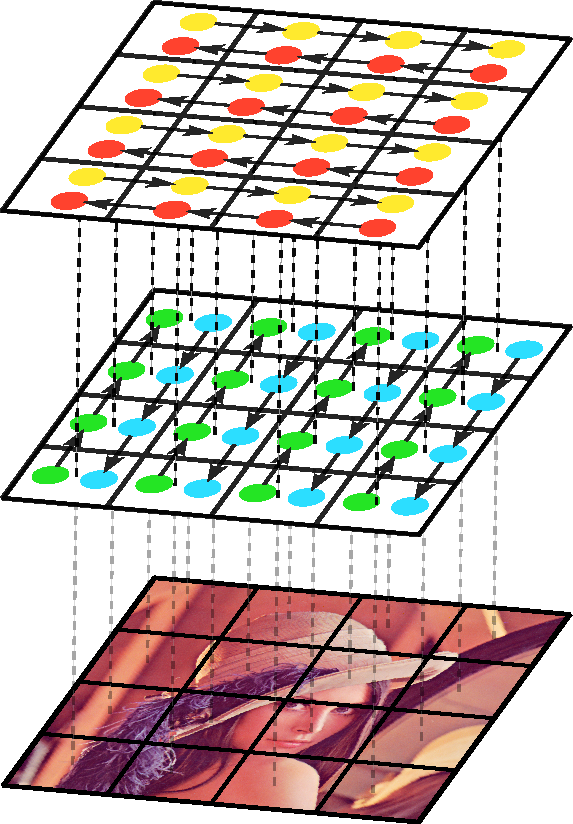
\includegraphics[width=0.3\columnwidth]{pdf/first_layer.pdf}
        \caption{A ReNet layer. The blue and green dots on the input
            image/feature map represent the steps of $f^{\downarrow}$ and
            $f^{\uparrow}$ respectively. On the concatenation of the resulting
            feature maps, $f^{\rightarrow}$ (yellow dots) and $f^{\leftarrow}$
            (red dots) are subsequently swept. Their feature maps are finally
            concatenated to form the output of the ReNet layer, depicted as a
            blue heatmap in the figure.}
        \label{fig:first_layer}
        \vspace{-5mm}
    \end{center}
\end{figure}


Specifically, the model takes as an input an image (or the feature map of the
previous layer) $\mathbf{X}$ of elements $x \in \RR^{H \times W \times C}$,
where $H$, $W$ and $C$ are respectively the height, width and number of
channels (or features) and splits it into $I \times J$ patches $p_{i,j} \in
\RR^{H_p \times W_p \times C}$. It then sweeps along each of its columns
$p_{i,\cdot}$ vertically a first time with two RNNs $f^{\downarrow}$ and
$f^{\uparrow}$, with $U$ recurrent units each, that move top-down and bottom-up
respectively. Note that the processing of each column is independent and can be
done in parallel. This is a very important performance difference of the ReSeg
model w.r.t. to other architectures in the literature that enforce to handle
the data in a more constrainedly sequential nature.

\begin{figure*}[t]
    \advance\leftskip-0.2\textwidth
    \centering
    \makebox[\textwidth][c]{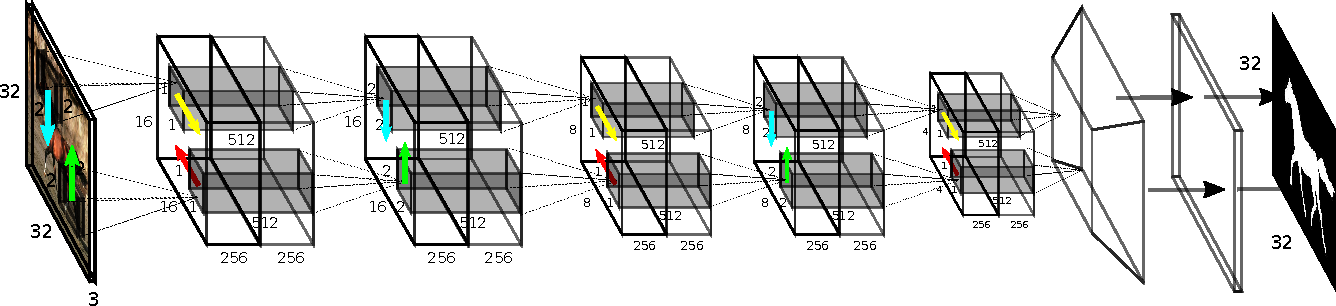
\includegraphics
    	[height=.135\textheight,width=\textwidth]{pdf/reseg_base.pdf}}
    \caption{The ReSeg network. For space reasons the pretrained VGG-16
        convolutional layers used to preprocess the input to ReSeg are
        not represented. The first 2 RNNs (blue and green) are applied on
        2x2x3 patches of the image, their 16x16x256 feature maps are
        concatenated and fed as input to the next two RNNs (red and yellow)
        which read 1x1x512 patches and emit the output of the first ReNet
        layer. Two similar ReNet layers are stacked, followed by an upsampling
        layer and a softmax nonlinearity.}
    \label{fig:ReSeg}
\end{figure*}

At every time step each RNN reads the next non-overlapping patch $p_{i,j}$ and,
based on its previous state, emits a projection $o_{i,j}^{\star}$ and updates
its state $z_{i,j}^{\star}$:
\begin{align}
    o^{\downarrow}_{i,j} = f^{\downarrow}(z^{\downarrow}_{i-1,j},p_{i,j}),
        &\text{ for }i=1,\cdots, I\\
    o^{\uparrow}_{i,j} = f^{\uparrow}(z^{\uparrow}_{i+1,j},p_{i,j}),
        &\text{ for }i=I,\cdots,1
\end{align}
It has to be stressed that the decision to read non-overlapping patches is a
modeling choice to increase the image scan speed and lower the memory usage,
but is not a limitation of the architecture.

Once the first two vertical RNNs have processed the whole input $X$, their
projections $o^{\downarrow}_{i,j}$ and $o^{\uparrow}_{i,j}$ are concatenated to
obtain a composite feature map $\mathbf{O^{\updownarrow}}$ whose elements
$o^{\updownarrow}_{i,j} \in \RR^{2U}$ can be seen as the activation of a
feature detector at the location $(i,j)$ with respect to all the patches in the
$j$-th column of the input. For simplicity, in the rest of this manuscript
this part of the model will be referred to as \emph{vertical recurrent
sublayer}.

After obtaining the concatenated feature map $\mathbf{O^{\updownarrow}}$, the
model sweeps over each of its rows with a pair of new RNNs $f^{\rightarrow}$ and
$f^{\leftarrow}$. Each element of $\mathbf{O^{\updownarrow}}$ is processed
individually, rather than grouping them into patches as was done in the vertical
recurrent sublayer. This was chosen so that the second recurrent sublayer has
the same spatial granularity as the first one, but this is not a constraint of
the model and different architectures can be explored.

With a similar but specular procedure as the one adopted for the first
sublayer, the network reads one element of the intermediate feature map
$o^\updownarrow_{i,j}$ at each step and emits two activations coming from two
new RNNs that are concatenated into a unique feature map
$\mathbf{O^\leftrightarrow}~=~\left\{ h^\leftrightarrow_{i,j} \right\}
_{i=1\dots I}^{j=1\dots J}$, with $o^\leftrightarrow_{i,j} \in
\RR^{2U}$. Each element $o^\leftrightarrow_{i,j}$ of this \emph{horizontal
recurrent sublayer} represents the features of one of the input image patches
$p_{i,j}$ \emph{with contextual information from the whole image}.

It is trivial to note that it is possible to concatenate many recurrent layers
$\mathbf{O^{(1 \cdots L)}}$ one after the other and train them with any
optimization algorithm that performs gradient descent, as the composite model
is a smooth, continuous function.

The recurrent layers that are the core of this architecture, can be either
implemented as vanilla $\tanh$ RNN layers, Gated Recurrent Unit~(GRU)
layers~\cite{Cho2014} or LSTM~layers~\cite{Hochreiter+Schmidhuber-1997}.
Previous work has shown that the ReNet model can perform well with little
concern for the specific recurrent unit used~\cite{visin2015renet}. The ReSeg
model was tested choosing GRU units over alternative implementations, as
they strike a good balance between memory usage and computational power, but
nothing prevents from using different kinds of RNN layers.

\subsection{Upsampling layer}\label{sec:upsampling}
Since by design each recurrent layer processes non-overlapping patches, the
size of the last composite feature map is smaller than the size of the
initial input $\mathbf{X}$, whenever the patch size is greater than one. To be
able to compute a segmentation mask at the same resolution as the ground truth,
the prediction has to be expanded back before applying the softmax
non-linearity.

Several different methods can be used to this end, e.g., fully connected
layers, full convolutions and transposed convolutions. The first is not a good
candidate in this domain as it does not take into account the topology of the
input, which is essential for this task; the second is not optimal either, as
it would require large kernels and stride sizes to upsample by the required
factor. Transposed convolutions are both memory and computation efficient, and
are the ideal method to tackle this problem.

Transposed convolutions -- also known as \emph{fractionally strided
convolutions} -- have been employed in many works in recent
literature~\cite{Zeiler-ICCV2011,ZeilerFergus14,long2015fully,
radford2015unsupervised,im2016generating}. This method is based on the observation
that direct convolutions can be expressed as a dot product between the
flattened input and a sparse matrix, whose non-zero elements are elements of the
convolutional kernel. The equivalence with the convolution is granted by the
connectivity pattern defined by the matrix.

Transposed convolutions apply the transpose of this transformation matrix to
the input, resulting in an operation whose input and output shapes are inverted
with respect to the original direct convolution. A very efficient implementation of
this operation can be obtained exploiting the gradient operation of the
convolution -- whose optimized implementation can be found in many of the most
popular libraries for neural networks. For an in-depth and comprehensive
analysis of each alternative,
%we refer the interested reader to~\cite{dumoulin2016guide}.
see~\autoref{sec:transposed_conv}.

\section{Experiments}\label{sec:reseg_experiments}

\subsection{Datasets}
We evaluated the proposed ReSeg architecture on several benchmark datasets.
We proceeded by first assessing the performances of the model on the Weizmann
Horse and the Oxford Flowers datasets and then focused on the more challenging
Camvid dataset. We will describe each dataset in detail in this section.

\subsubsection{Weizmann Horse}
The Weizmann Horse dataset, introduced in~\cite{Borenstein04combiningtop-down},
is an image
segmentation dataset consisting of 329 variable size images in both RGB and
gray scale
format, matched with an equal number of groundtruth segmentation images, of
the same size as the corresponding image.
The groundtruth segmentations contain a foreground/background mask of the
focused horse, encoded as a real-value between 0 and 255. To convert this into
a boolean mask, we threshold in the center of the range setting all smaller
values to 0, and all greater values to 1.
%This dataset is one of the primary
%small-scale benchmarks found in existing image segmentation literature.

% \subsubsection{Fashionista}
% The Fashionista dataset from ~\cite{Fashionista} contains 685 RGB images of
% fashion models wearing a variety of different clothing.
% Each image and its corresponding mask are 400 pixels in width by 600 pixels
% in height, with encoded values for 53 clothing items. In this work we focus
% on foreground/background segmentation, and build the appropriate
% masks from the more complex maps provided by the dataset by creating a new map
% which preserves the background class as 0, and sets pixels which belong to all
% other classes to 1. This appears to be the same procedure undertaken in
% ~\cite{yang2015patchcut} to create a foreground/background task for this dataset.

\subsubsection{Oxford Flowers 17}
The Oxford Flowers 17 class dataset from~\cite{Nilsback06} contains 1363
variable size RGB images, with 848 image segmentations maps associated with
a subset of
the RGB images. There are 8 unique segmentation classes defined over all maps,
including flower, sky, and grass. To build a foreground/background mask,
we take the original segmentation maps, and set any pixel not belonging to
class 38 (flower class) to 0, and setting the flower class pixels to 1.
This binary segmentation task for Oxford Flowers 17 is further described
in~\cite{Xiaomeng14}.
%A larger 102 class Oxford Flowers dataset is available from the same authors.

\subsubsection{CamVid Dataset}
The Cambridge-driving Labeled Video Database
(CamVid)~\cite{Brostow2010semantic} is a real-world dataset which consists of
images recorded from a car with an internally mounted camera, capturing frames
of $960 \times 720$ RGB pixels per frame, with a recording frame rate of 30
frames per second. A total of ten minutes of video was recorded, and
approximately one frame per second has been manually annotated with per pixel
class labels, from one of 32 possible classes.  A small number of pixels were
labelled as void in the original dataset. These do not belong to any of the 32
classes prescribed in the original data, and are ignored during evaluation.  We
used the same subset of 11 class categories as~\cite{badrinarayanan2015segnet}
for experimental analysis.  The CamVid dataset itself is split into 367
training, 101 validation and 233 test images, and in order to make our
experimental setup fully comparable to~\cite{badrinarayanan2015segnet}, we
downsampled all the images by a factor of 2 resulting in a final $480 \times
360$ resolution.

% \subsection{Preprocessing}\label{sec:data_preprocessing}
% \subsubsection{Data Augmentation}
% Adding prior knowledge by augmenting the given data with transformed versions is
% well known to help generalization ~\cite[see, e.g.,][]{Krizhevsky-2012}. In light
% of this, we decided to employ several methods of data augmentation:
% {\it flipping}, {\it shifting}, {\it color flipping}, and {\it resizing}.
%
% For each sample there was a 50\% chance to flip the image horizontally.
% This mirrors the intuition that images which are inverted horizontally
% generally seem like the same scene visually.
%
% The shifting procedure was as follows: we either move 2 pixels to the left with
% 25\% chance, 2 pixels to the right with 25\% chance, or perform no shifting.
% After this step, we then shift up with 25\% chance, shift down with 25\% chance,
% or leave the image as is was before this step. This augmentation should make
% the model more robust to slight shifts of the object in the image.
%
% When working with gray-scale images, another augmentation which can be useful
% is to randomly invert the color of the image by changing darker colors into lighter
% colors, and vice-versa. This proved to be especially helpful
% when working with greyscale versions of the Weizmann Horse dataset to improve the segmentation
% performance of light horses that are less represented in the dataset.
%
% Resizing of images can also be of benefit, as eliminating unnecessary and
% easily explained variance can help the model focus on harder to model
% characteristics, which generally leads to better performance on the task at hand,
% especially in the case of segmentation where object scale between images has little
% impact on the class category. A common choice for resizing is to resize every image
% to the mean width and height, calculated over the entire dataset of variable size
% images.
%
% It should be noted that all transformations which involve changes in dimensionality
% or position must also be applied in some form to the segmentation mask, and great
% care must be taken (especially during resizing/shifting) not to introduce unexpected
% errors. It is also paramount to highlight that it is the prediction that
% should be resized to the ground truth size and not the opposite, not
% to misrepresent the segmentation accuracy.
%
% All of these possible augmentation procedures were treated as hyperparameters for
% training, and selected based on the best validation performance per dataset.

\begin{table*}[!ht]
    % HORSES
    \begin{minipage}{0.45\textwidth}
        \centering
        \small{%
            \begin{tabular}{c|c|c||c|c|c}
                \multicolumn{1}{c}{Method} & \multicolumn{1}{c}{Global acc} & \multicolumn{1}{c}{\textbf{Avg IoU}}\\ \hline \hline

                All foreground baseline & 25.4 & 79.9 \\ \hline
                All background baseline & 74.7 & 0.0 \\ \hline
                Kernelized structural SVM \cite{bertelli2011kernelized} & 94.6 & 80.1 \\ \hline
                ReSeg (no VGG) & 94.9 & 79.9 \\ \hline
                CRF learning \cite{liu2015crf} & 95.7 & 84.0 \\ \hline
                PatchCut \cite{yang2015patchcut} & 95.8 & 84.0 \\ \hline
                \textbf{ReSeg} & 96.8 & \textbf{91.6} \\ \hline

            \end{tabular}
            \vspace*{0.1cm}
        }
        \caption{Weizmann Horses. Per pixel accuracy and IoU are
            reported.}
        \label{tbl:WeizmannHorses_SOTA}
    \end{minipage}
    \quad
    % FLOWERS
    \begin{minipage}{0.45\textwidth}
        \centering
        \small{%
            \begin{tabular}{c|c|c||c|c|c}
                \multicolumn{1}{c}{Method} & \multicolumn{1}{c}{Global acc} & \multicolumn{1}{c}{\textbf{Avg IoU}}\\ \hline \hline

                All background baseline & 71.0 & 0.0 \\ \hline
                All foreground baseline & 29.0 & 29.2 \\ \hline
                % \textbf{ReSeg (no VGG)} & 86.9 & \textbf{65.8} \\ \hline
                GrabCut \cite{rother2004grabcut} & 95.9 & 89.3 \\ \hline
                Tri-map \cite{Xiaomeng14} & 96.7 & 91.7 \\ \hline
                \textbf{ReSeg} & 98 & \textbf{93.7} \\ \hline

            \end{tabular}
            \vspace*{0.1cm}
        }
        \caption{Oxford Flowers. Per pixel accuracy and IoU are
            reported.}
        \label{tbl:OxfordFlowers_SOTA}
    \end{minipage}
\end{table*}

% CAMVID RESULTS
\begin{table*}[!ht]
	\resizebox{\textwidth}{!}{%
		\small{%
            \begin{tabular}{c|c|c|c|c|c|c|c|c|c|c|c||c|c|c}

                \multicolumn{1}{c}{Method} & \multicolumn{1}{c}{\rotatebox{90}{Building}} & \multicolumn{1}{c}{\rotatebox{90}{Tree}} & \multicolumn{1}{c}{\rotatebox{90}{Sky}} & \multicolumn{1}{c}{\rotatebox{90}{Car}} & \multicolumn{1}{c}{\rotatebox{90}{Sign-Symbol}} & \multicolumn{1}{c}{\rotatebox{90}{Road}} & \multicolumn{1}{c}{\rotatebox{90}{Pedestrian}} & \multicolumn{1}{c}{\rotatebox{90}{Fence}} & \multicolumn{1}{c}{\rotatebox{90}{Column-Pole}} & \multicolumn{1}{c}{\rotatebox{90}{Side-walk}} & \multicolumn{1}{c}{\rotatebox{90}{Bicyclist}} & \multicolumn{1}{c}{\rotatebox{90}{Avg class acc}} & \multicolumn{1}{c}{\rotatebox{90}{Global acc}} & \multicolumn{1}{c}{\rotatebox{90}{\textbf{Avg IoU}}}\\ \hline \hline

				\multicolumn{15}{c}{\emph{Segmentation models}} \\ \hline
                Super Parsing   \cite{tighe2013superparsing} & \textbf{87.0} & 67.1 & \textbf{96.9} & 62.7 & 30.1 & 95.9 & 14.7 & 17.9 & 1.7 & 70.0 & 19.4 & 51.2 & 83.3 & n/a \\ \hline
				Boosting+Higher order \cite{sturgess2009combining} & 84.5 & 72.6 & \textbf{97.5} & 72.7 & 34.1 & 95.3 & 34.2 & 45.7 & 8.1 & 77.6 & 28.5 & 59.2 & 83.8 & n/a \\ \hline
				Boosting+Detectors+CRF \cite{ladicky2010and} & 81.5 & 76.6 & 96.2 & 78.7 & 40.2 & 93.9 & 43.0 & 47.6 & 14.3 & 81.5 & 33.9 & 62.5 & 83.8 & n/a \\ \hline

				\multicolumn{15}{c}{\emph{Neural Network based segmentation models}} \\ \hline
				SegNet-Basic (layer-wise training \cite{badrinarayanan2015segnetlayerwise}) & 75.0 & 84.6 & 91.2 & 82.7 & 36.9 & 93.3 & 55.0 & 37.5 & 44.8 & 74.1 & 16.0 & 62.9 & 84.3 & n/a \\ \hline
                SegNet-Basic \cite{badrinarayanan2015segnet} & 80.6 & 72.0 & 93.0 & 78.5 & 21.0 & 94.0 & 62.5 & 31.4 & 36.6 & 74.0 & 42.5 & 62.3 & 82.8 & 46.3 \\ \hline
                SegNet \cite{badrinarayanan2015segnet} & \textbf{88.0 } & \textbf{87.3} & 92.3 & 80.0 & 29.5 & \textbf{97.6} & 57.2 & \textbf{49.4} & 27.8 & 84.8 & 30.7 & 65.9 & 88.6 & 50.2 \\ \hline
                \emph{ReSeg + Class Balance} & 70.6 & 84.6 & 89.6 & 81.1 & \textbf{61.0} & 95.1 & \textbf{80.4} & 35.6 & \textbf{60.6} & \textbf{86.3} & \textbf{60.0} & 73.2 & 83.5 & 53.7 \\ \hline
                \textbf{ReSeg} & 86.8 & 84.7 & 93.0 & \textbf{87.3} & 48.6 & \textbf{98.0} & 63.3 & 20.9 & 35.6 & \textbf{87.3} & 43.5 & 68.1 & 88.7 & \textbf{58.8} \\ \hline

				\multicolumn{15}{c}{\emph{Sub-model averaging}} \\ \hline
                \emph{Bayesian SegNet-Basic} \cite{Kendall2015bayesiansegnet} & 75.1 & 68.8 & 91.4 & 77.7 & 52.0 & 92.5 & 71.5 & 44.9 & 52.9 & 79.1 & 69.6 & 70.5 & 81.6 & 55.8 \\ \hline
                \emph{Bayesian SegNet} \cite{Kendall2015bayesiansegnet} & 80.4 & 85.5 & 90.1 & 86.4 & 67.9 & 93.8 & 73.8 & 64.5 & 50.8 & 91.7 & 54.6 & 76.3 & 86.9 & 63.1 \\ \hline

			\end{tabular}
		}
    }
	\vspace*{0.1cm}
    \caption{%
        CamVid. The table reports the per-class accuracy, the average per-class
        accuracy, the global accuracy and the average intersection over union.
        The best values and the values within $1$ point from the best are
        highlighted in bold for each column. For completeness we report the
        Bayesian Segnet models even if they are not directly comparable to the
        others as they perform a form of model averaging.}
    \label{tbl:camvid_SOTA}
\end{table*}

% CAMVID PARAMS
\begin{table*}[!ht]
    \resizebox{\textwidth}{!}{%
        \small{%
            \begin{tabular}{c|c|c|c|c|c|c|c|c|c|c|c|c|c|c|c||c|c|c}
                \multicolumn{1}{c}{Model} & \multicolumn{1}{c}{${ps}_{\text{RE}}$}& \multicolumn{1}{c}{$d_{\text{RE}}$} & \multicolumn{1}{c}{${fs}_{\text{UP}}$}& \multicolumn{1}{c}{$d_{\text{UP}}$} & \multicolumn{1}{c}{\rotatebox{90}{Building}} & \multicolumn{1}{c}{\rotatebox{90}{Tree}} & \multicolumn{1}{c}{\rotatebox{90}{Sky}}  & \multicolumn{1}{c}{\rotatebox{90}{Car}}  & \multicolumn{1}{c}{\rotatebox{90}{Sign-Symbol}} & \multicolumn{1}{c}{\rotatebox{90}{Road}} & \multicolumn{1}{c}{\rotatebox{90}{Pedestrian}} & \multicolumn{1}{c}{\rotatebox{90}{Fence}} & \multicolumn{1}{c}{\rotatebox{90}{Column-Pole}} & \multicolumn{1}{c}{\rotatebox{90}{Side-walk}} & \multicolumn{1}{c}{\rotatebox{90}{Bicyclist}} & \multicolumn{1}{c}{\rotatebox{90}{Avg class acc}} & \multicolumn{1}{c}{\rotatebox{90}{Global acc}} & \multicolumn{1}{c}{\rotatebox{90}{\textbf{Avg IoU}}}\\ \hline \hline

                ReSeg + LCN & $(2 \times 2), (1 \times 1)$ & (100, 100) & $(2 \times 2)$ & (50, 50) & 81.5 & 80.3 & \textbf{94.7} & 78.1 & 42.8 & \textbf{97.4} & 53.5 & 34.3 & 36.8 & 68.9 & 47.9 & 65.1 & 84.8 & 52.6 \\ \hline
                ReSeg + Class Balance & $(2 \times 2), (1 \times 1)$ & (100, 100) & $(2 \times 2)$ & (50, 50) & 70.6 & \textbf{84.6} & 89.6 & 81.1 & \textbf{61.0} & 95.1 & \textbf{80.4} & \textbf{35.6} & \textbf{60.6} & \textbf{86.3} & \textbf{60.0} & 73.2 & 83.5 & 53.7 \\ \hline
                \textbf{ReSeg} & $(2 \times 2), (1 \times 1)$ & (100, 100) & $(2 \times 2)$ & (50, 50) & \textbf{86.8} & \textbf{84.7} & 93.0 & \textbf{87.3} & 48.6 & \textbf{98.0} & 63.3 & 20.9 & 35.6 & \textbf{87.3} & 43.5 & 68.1 & 88.7 & \textbf{58.8} \\ \hline
            \end{tabular}%
        }
    }
    \vspace*{0.1cm}
    \caption{%
        Comparison of the performance of different hyperparameter on CamVid.
    }
    \label{tbl:camvid_params}
\end{table*}

\subsection{Experimental settings}
To gain confidence with the sensitivity of the model to the different
hyperparameters, we decided to evaluate it first on the Weissman Horse and
Oxford Flowers datasets on a binary segmentation task; we then focused the most
of our efforts on the more challenging semantic segmentation task on the CamVid
dataset.

The number of hyperparameters of this model is potentially very high, as for
each ReNet layer different implementations are possible (namely vanilla RNN,
GRU or LSTM), each one with its specific parameters. Furthermore, the number of
features, the size of the patches and the initialization scheme have to be
defined for each ReNet layer as well as for each transposed convolutional
layer. To make it feasible to explore the hyperparameter space, some of the
hyperparameters have been fixed by design and the remaining have been finetuned.
In the rest of this section, the architectural choices for both sets of
parameters will be detailed.

All the transposed convolution upsampling layers were followed by a
ReLU~\cite{Krizhevsky2012-alexnet} non-linearity and initialized with the
fan-in plus fan-out initialization scheme described
in~\cite{glorot2010understanding}. The recurrent weight matrices were instead
initialized to be orthonormal, following the procedure defined
in~\cite{Saxe2014}. We also constrained the stride of the upsampling transposed
convolutional layers to be tied to their filter size.

In the segmentation task, each training image carries classification
information for all of its pixels. Differently from the image classification
task, small batch sizes provide the model with a good amount of information
with sufficient variance to learn and generalize well. We experimented with
various batch sizes going as low as processing a single image at the time,
obtaining comparable results in terms of performance. In our experiments we
kept a fixed batch size of $5$, as a compromise between train speed and memory
usage. In all our experiments, we used L2
regularization~\cite{Krogh92asimple}, also known as weight decay, set to
$0.001$ to avoid instability at the end of training. We trained all our models
with the Adadelta~\cite{Zeiler-2012} optimization algorithm, for its desired
property of not requiring a specific hyperparameter tuning. The effect of Batch
Normalization in RNNs has been a focus of attention~\cite{Laurent2015}, but it
does not seem to provide a reliable improvement in performance, so we decided
not to adopt it.
% we did not use any gradient clipping or weight noise.

In the experiments, we varied the number of ReNet layers and the number of
upsampling transposed convolutional layers, each of them defined respectively
by the number of features $d_{\text{RE}}(l)$ and $d_{\text{UP}}(l)$,
the size of the input patches (or equivalently of the filters)
${ps}_{\text{RE}}(l)$ and ${fs}_{\text{UP}}(l)$.

% \begin{table}[ht]
%
%     \centering
%     \caption{Hyperparameters} \label{tbl:hyperparams}
%     \begin{tabular}{l | l | l | l | l | l | l | l}
%         Dataset & $b$ & $d_{\text{RE}}$ & $w_p$ & $h_p$ & $a_c$ &
%         upscaling\\
%         \hline
% Weissman horses & 1 & [1100, 1300] & 2 & 2 & tanh & grad \\
% Fashonista & 1 & [400, 400] & 2 & 2 & tanh & linear \\
% Oxford Flowers & 5 & [150, 150] & 2 & 2 & tanh & linear
%     \end{tabular}
%     \vspace{2mm}
% \end{table}


% An adaptive learning rate algorithm known as Adam~\cite{Kingma2014} was a
% key ingredient to stable learning, though others such as ~\cite{Zeiler-2012}
% were useful during model development. In addition, we also utilized
% gradient norm rescaling to help with the problems described in
% ~\cite{bengio2013advances}.
%
% Regularization proved to be another important part of our process,
% especially on the smaller Weizmann Horse dataset. Weight noise, as described
% in ~\cite{Graves2011}, with a scale 0.075 was applied to all weight matrices
% before each forward pass during some experiments. Dropout ~\cite{Srivastava14} on
% each forward connection with drop probability of $0.2$ on the input, and/or with drop
% probability of $0.5$ on the hidden projections was applied during some experiments.
% Many experiments were performed using a minibatch size of 1. When computational
% constraints allowed, we also used larger batch sizes of 5, 10, 20, 35, and 50.
% Larger batch sizes greatly smoothed learning (as expected), and removed some
% issues related to spurious occurrences in the datasets such as misaligned or
% poorly segmented groundtruth masks.

\subsection{Results}

In~\autoref{tbl:WeizmannHorses_SOTA}, we report the results on the Weizmann
Horse dataset. On this dataset, we verified the assumption that processing
the input image with some pre-trained convolutional layers from VGG-16 could
ease the learning. Specifically, we restricted ourselves to only using the
first $7$ convolutional layers from VGG, as we only intended to extract some
low-level generic features and learn the task-specific high-level features with
the ReNet layers. The results indeed show an increase in terms of average Intersection
over Union (\emph{IoU}) when these layers are being used, confirming our
hypothesis.

\autoref{tbl:OxfordFlowers_SOTA} shows the results for Oxford Flowers
dataset, when using the full ReSeg architecture (i.e., including VGG convolutional layers).
As shown in the table, our method clearly outperforms the
state-of-the-art both in terms of global accuracy and average IoU.

\autoref{tbl:camvid_SOTA} presents the results on CamVid dataset using the full
ReSeg architecture. Our model exhibits state-of-the-art performance in terms of
IoU when compared to both standard segmentation methods and neural network
based methods, showing an increase of $17\%$ w.r.t.\ to the recent SegNet
model. It is worth highlighting that incorporating sub-model averaging to
SegNet model, as in \cite{Kendall2015bayesiansegnet}, boosts the original model
performance, as expected. Therefore, introducing sub-model averaging to ReSeg
would also presumably result in significant performance increase.  However,
this remains to be tested.

% There are number of difficulties in directly comparing our performance with the
% reported scores, some of which are intrinsic to using neural based models for
% segmentation, while others are specific to the evaluation datasets or competing
% methodologies.

%\begin{figure}[t]
%    \centering
%    \makebox[\columnwidth][c]{\includegraphics[width=1.1\columnwidth]
%    {Segm_horse258.pdf}}
%    \caption{Weizmann Horse example segmentation.
%        Left: Input image, Center: Ground truth segmentation,
%        Right: ReSeg predicted segmentation}
%    \label{fig:ReSeg_example}
%\end{figure}

%\begin{figure}[t]
%    \centering
%    \makebox[\columnwidth][c]{\includegraphics[width=1.1\columnwidth]
%    {Segm_horse283.pdf}}
%    \caption{Weizmann Horse failure segmentation.
%        Left: Input image, Center: Ground truth segmentation,
%        Right: ReSeg predicted segmentation}
%    \label{fig:ReSeg_failure}
%\end{figure}

\section{Conclusions/Discussion}

As reported in the previous section, our experiments on the Weizmann Horse
dataset show that processing the input images with some layers of VGG-16
pre-trained network improves the results. In this setting, pre-processing the input
with Local Contrast Normalization (LCN) does not seem to give any advantage
(see~\autoref{tbl:camvid_params}). We did not use any other kind of
pre-processing.

While on both the Weizmann Horse and the Oxford Flowers datasets we trained on
a binary background/foreground segmentation task, on CamVid we addressed the
full semantic segmentation task. In this setting, when the dataset is highly
imbalanced, the segmentation performance of some classes can drop
significantly as the network tries to maximize the score on the high-occurrence
classes, {\em de facto} ignoring the low-occurrence ones. To overcome this behaviour,
we added a term to the cross-entropy loss to bias the prediction towards the
low-occurrence classes. We use \emph{median frequency
balancing}~\cite{Eigen2015}, which re-weights the class predictions by the
ratio between the median of the frequencies of the classes (computed on the
training set) and the frequency of each class.
% \begin{equation}
% \alpha(c) = median\_frequency / f(c)
% \end{equation}
% where $f(c)$  is the number of pixels of the class $c$ divided by the total
% number of pixels in the images where $c$ is present, and $median\_frequency$ is
% the median of these frequencies.
This increases the score of the low frequency classes
(see~\autoref{tbl:camvid_params}) at the price of a more noisy segmentation
mask, as the probability of the underrepresented classes is overestimated and
can lead to an increase in misclassified pixels in the output segmentation
mask, as shown in~\autoref{fig:camvid_class_balance}.

On all datasets we report the per-pixel accuracy (\emph{Global acc}), computed
as the percentage of true positives w.r.t.\ the total number of pixels in the
image, and the average per-class Intersection over Union (\emph{Avg IoU}),
computed on each class as true positive divided by the sum of true positives,
false positives and false negatives and then averaged. In the full semantic
segmentation setting we also report the per-class accuracy and the average
per-class accuracy (\emph{Avg class acc}).

\begin{figure*}[!htb]
    \centering
    % \makebox[\textwidth][c]{
    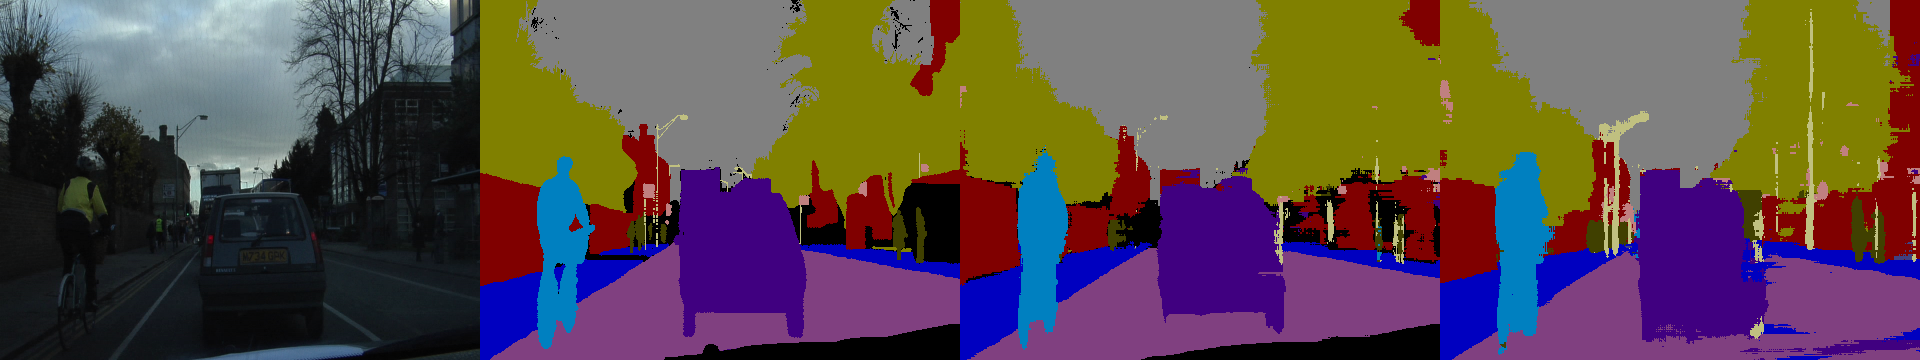
\includegraphics[width=\textwidth]{img/camvid_classbal_diff.png}%}
    \caption{Camvid segmentation example with and without class balancing. From
        the left: input image, ground truth segmentation, ReSeg segmentation,
        ReSeg segmentation with class balancing. Class balancing improves the
        low frequency classes as e.g., the street lights, at the price of a
        worse overall segmentation.}
    \label{fig:camvid_class_balance}
\end{figure*}

\section{Conclusion}
We introduced the ReSeg model, an extension of the ReNet model for image
semantic segmentation. The proposed architecture shows state-of-the-art
performances on CamVid, a widely used dataset for urban scene semantic
segmentation, as well as on the much smaller Oxford Flowers dataset. We also
report state-of-the-art performances on the Weizmann Horses.

In our analysis, we discuss the effects of applying some layers of VGG-16 to
process the input data, as well as those of introducing a class balancing
term in the cross-entropy loss function to help the learning of
under-represented classes.
Notably, it is sufficient to process the input images with just a few layers of
VGG-16 for the ReSeg model to gracefully handle the semantic segmentation task, confirming
its ability to encode contextual information and long term dependencies.
